%%%%% Inspection and Characterization Plan for DESC

%----------------------------------------------------------------------------------------
%	PACKAGES AND DOCUMENT CONFIGURATIONS
%----------------------------------------------------------------------------------------

\documentclass[12pt, a4paper]{article}

\usepackage{graphicx} % Required for the inclusion of images
\usepackage{natbib} % Required to change bibliography style to APA
\usepackage{amsmath} % Required for some math elements 

\setlength\parindent{0pt} % Removes all indentation from paragraphs

%\usepackage{times} % Uncomment to use the Times New Roman font

%----------------------------------------------------------------------------------------
%	DOCUMENT INFORMATION
%----------------------------------------------------------------------------------------

\title{Inspection and Characterization Plan} % Title

\author{Science Release and Validation team} % Author name

\date{\today} % Date for the report

\begin{document}

\maketitle % Insert the title, author and date

\begin{center}
Version 0.2
\end{center}

% If you wish to include an abstract, uncomment the lines below
% \begin{abstract}
% Abstract text
% \end{abstract}

%----------------------------------------------------------------------------------------
%	SECTION 1 -- the document's purpose is described, plus reference info
%----------------------------------------------------------------------------------------

\section{Purpose of the document}

This document is aimed at describing the process to execute the test suite necessary to characterize new Rubin data releases, in the context of the DESC. It covers the following points:

\begin{itemize}
\item Describe the goal of characterization tests for DESC.
\item The list of tests, methods, tools and criteria (where applicable) to characterize and validate the Rubin dataset, for the purposes of DESC analyses.
\item The actual procedure for the execution of tests and inspection.
\end{itemize}

%\subsection{Changes from the last version}

\subsection{Definitions, reference documents}

\begin{itemize}
\item Test run: a single execution of the whole SRV characterization framework. Includes tests using DESCQA, other sources, inspection of data and documentation.
\item Test Execution Report (TER): a short document where the results of a Test run are summarized.
\end{itemize}
 
%----------------------------------------------------------------------------------------
%	SECTION 2 -- the purpose of the test runs is described
%----------------------------------------------------------------------------------------
\section{Goals of the characterization process}

The overall objective of the inspection and characterization procedure is to \textbf{provide a compiled snapshot of the characteristics of the data}. This can respond to three needs:

\begin{itemize}
	\item Provide a repository of the status of the data set used for the DESC science analyses, used as reference for understanding the results and reporting on papers. This requires a lower frequency of runs (months time scale)
	\item Explore characteristics of different science samples, within the same data release (weeks time scale)
	\item Assess issues with the data release, for DESC purposes (days time scale)
\end{itemize}

It is expected that the Rubin project will provide, alongside with the data itself, documentation and/or reports on the data quality, conducted by their own Verification and Validation tests. With the framework that SRV is providing here, the intention is to cater to the interests of the DESC ('fill the gaps'), in case some tests are missing from those provided by Rubin, evaluating the characteristics of 'typical' DESC science samples, testing DESC only value added products, and rechecking some basic metrics in case the data source is different than that of the Rubin Science Platform (e.g., if DESC uses a subset of the data in a different platform or format at NERSC).

A structured compilation of all the relevant tests and inspections will be finally recorded on static Test Execution Reports, which should contain all the information necessary for provenance and regression purposes.

At the same time, it is noteworthy to consider that the execution of these tests are easily run and re-run, and do not require a significant overhead in terms of execution and SRV (DESC) scientists' time, so as to make this framework useful as a quick assessment. A final overall evaluation of the data quality for a 'frozen' version of the data release can be done with a more comprehensive approach, as a final report usable as reference for downstream analyses. Therefore, any science done would be able to use the corresponding TER metrics and references, and minimize any ambiguities as to which version of the data or catalog content is used.

The overall characterization framework is sketched in Figure \ref{fig:srvplanning} and summarized below. The tests referred will be described in this document:

\begin{enumerate}
	\item Data is made visible for an official Release at the Science Platform. It is foreseen that part of this data is copied to NERSC. At this point, \textbf{inspection tests} through Jupyter notebooks can be performed quickly to assess overall data health. Examples: RA,DEC coverage; histograms of flags; other simple histograms of the main photometric quantities. It is interesting to verify whether the results are compatible at the Rubin Science Platform and at NERSC. This inspection \textit{could} be complemented by tests being run through other tools, if that seems to be more manageable (examples: running TOPCAT and acquiring data from the Rubin Science Platform through TAP, using Lite IDACs capabilities such as those from Hadoop frameworks holding a version of the data). In all cases, the tests have to be formalized to ensure proper provenance.
	\item At the same time, the presence of \textbf{adequate documentation} from Rubin side for DESC purposes, can be inspected, complementing it when appropriate or reporting back to the project.
	\item \textbf{Main software tests will be run through a single framework (DESCQA)}.
	\item Tests already embedded in pre-existing frameworks, or coming from downstream analyses are included through DESCQA in the final report, ensuring consistency of the data sets used for the tests, with respect to those developed specifically in the previous point.
	\item Finally, besides the TER static reporting, DESCQA will provide \textbf{visualization utilities} for the test runs and re-runs that will inform the contents of the TER.
\end{enumerate}

\begin{figure}[h]
\begin{center}
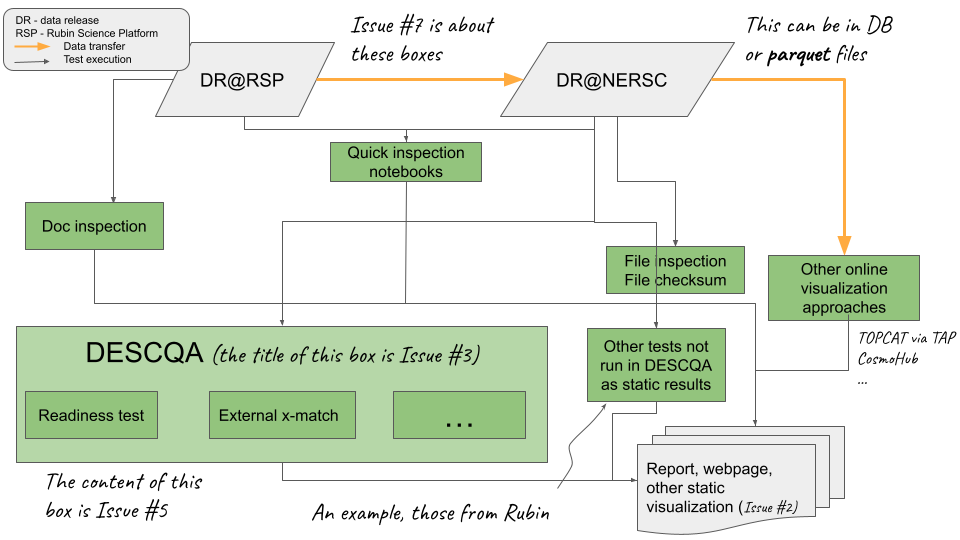
\includegraphics[width=0.95\textwidth]{../SRV_planning_diagram.png} 
\caption{SRV planning diagram}
\label{fig:srvplanning}
\end{center}
\end{figure}



%----------------------------------------------------------------------------------------
%	SECTION 3 -- the software and other tools are described
%----------------------------------------------------------------------------------------

\section{Test tool description}

Here we include an overall view of the software involved in a single test run of the SRV characterization framework.

\subsection{Software tools}

\textit{A list of references to the software used. The Test Execution Reports will be filled out with the actual versions and other specifics. These will be mainly pointers to GitHub repos holding the code to be executed.}

The main software tool is based on DESCQA\footnote{https://github.com/LSSTDESC/descqa}, a framework to validate simulated galaxy catalogs.

\subsection{Data sets and formats}

\textit{An explanation of the characteristics of the model of the data set being tested.}

\subsubsection{DC2}

DC2 coadd catalogs are available as flat parquet files at NERSC. \textit{The TER should include the actual location and details of the data that was used specifically.}

\subsubsection{DP0.2}

DP0.2 coadd catalogs are available as flat parquet files at NERSC. \textit{The TER should include the actual location and details of the data that was used specifically.}

%----------------------------------------------------------------------------------------
%	SECTION 4 -- the specific characterization cases and procedures are described
%----------------------------------------------------------------------------------------

\section{Characterization cases and procedures}

\subsection{Quick inspection notebooks}
Interactive notebooks to be included here that complement or substitute DESCQA executions, that could be run on NERSC and RSP. Also CosmoHub could be an option if the data is available.

\subsection{Documentation inspection}
Describe what documentation should be present to understand the data.

\subsection{Characterization of data set through DESCQA}

%\subsubsection{TC1 - Checks on catalog columns}
%\textbf{Purpose:} 

%Verify that the catalogs contain the columns we need.

%\textbf{Strategy:} 

%Execute an interactive job over the whole data set of the ColumnInspection test from DESCQA.

%This can be a simple listing of all columns, and making an automatic check on whether certain columns exist or not. 
%Another part can check for NaNs or crazy values in the relevant columns (similar to what the Readiness test does in DESCQA)

%\textbf{Procedure:} 

%Describe how we actually go about running this (./descqarun --t ColumnInspection --c DC2 etc.). Inputs and outputs.

%\subsubsection{TC2 - Statistics on sample selection}
%\textbf{Purpose:} 

%Compute the number of objects after various subselections, based on Rubin or DESC flags or quantity filters.

%\textbf{Strategy:} 

%Run a count test on coadd catalogs, and build a bar plot for each sample after passing subsequent cuts.

%\textbf{Procedure:} 

%Describe how we actually go about running this (./descqarun --t SampleStatistics --c DC2 etc.)


\subsubsection{TC1 - Readiness tests}
\textbf{Purpose:} 

Run a general 'readiness' test on coadd catalogs, to verify that there aren't any significant issues in data. Plot histograms and scatter plots of listed quantities and perform range, finiteness, mean and standard deviation checks.

\textbf{Strategy:} 

Execute an interactive job of the srv\_readiness test from DESCQA. These should be done on the overall data set.  \textit{Eventually, subsamples can be explored as well}.

The test currently comprises the following checks:
\begin{itemize}
	\item RA,DEC plot. Check that the footprint in the range expected by the associated data release documentation.
	\item Differential magnitude histograms in all ugrizy bands, for PSF, aperture and model magnitudes. Check that the depth is in the range expected by the associated documentation.
	%\item Magnitude vs magnitude error scatter plots of the above. Check that the depth is in the range expected by the associated documentation.
	%\item Color-color plots (specifics TBC). Is the stellar locus clearly visible, extended sources in the adequate range according to the redshift expected from the associated documentation.
	%\item Magnitude vs size plots fpr PSF-like objects. Are there significant outliers or biases.
	%\item PSF ellipticity whisker plot
	%\item Source e1,e2 histogram (TBC, requires some source selection)
\end{itemize}

\textbf{Procedure:} 

\begin{enumerate}
	\item Create a memory allocation on a NERSC node: salloc -N 1 -C haswell -{}-qos=interactive -t 02:00:00
	\item From the descqa directory (check version and state on TER), execute ./run\_master\_parallel.sh -v -c [catalog name] -t srv\_readiness. 
	\item Fill in TER for code version and tested catalog.
\end{enumerate}

\subsubsection{TC2 - Shape-related characterization}
\textbf{Purpose:} 

Run a few diagnostics on core measurements of the shapes on each band. 

\textbf{Strategy:} 

Execute an interactive job of the srv\_shear test from DESCQA. These should be done on the overall data set.  \textit{Eventually, subsamples can be explored as well}.

The test currently comprises the following checks:
\begin{itemize}
	\item Ellipticity plot. 
	\item Moments plot.
	\item PSF plot.
	%\item Color-color plots (specifics TBC). Is the stellar locus clearly visible, extended sources in the adequate range according to the redshift expected from the associated documentation.
	%\item Magnitude vs size plots fpr PSF-like objects. Are there significant outliers or biases.
	%\item PSF ellipticity whisker plot
	%\item Source e1,e2 histogram (TBC, requires some source selection)
\end{itemize}

\textbf{Procedure:} 

\begin{enumerate}
	\item Create a memory allocation on a NERSC node: salloc -N 1 -C haswell -{}-qos=interactive -t 02:00:00
	\item From the descqa directory (check version and state on TER), execute ./run\_master\_parallel.sh -v -c [catalog name] -t srv\_shear. 
	\item Fill in TER for code version and tested catalog.
\end{enumerate}

\subsubsection{TC3 - Galaxy density}
\textbf{Purpose:} 

Measure number of galaxies per square arcmin after successive quality cuts. Plot their sky distribution and write global statistics.

\textbf{Strategy:} 

Execute an interactive job over the whole data set of the srv\_ngals test from DESCQA. 

\textbf{Procedure:} 

\begin{enumerate}
	\item Create a memory allocation on a NERSC node: salloc -N 1 -C haswell -{}-qos=interactive -t 02:00:00
	\item From the descqa directory (check version and state on TER), execute ./run\_master\_parallel.sh -v -c [catalog name] -t srv\_ngals. 
	\item Fill in TER for code version and tested catalog.
\end{enumerate}

\subsubsection{TC4 - TXPipe results}
Incorporate TXPipe results of tests on the same data set that will complement this report.

\textbf{Strategy:} 

Execute an interactive job over the whole data set of the ExternalTest test from DESCQA. 

\textbf{Procedure:} 

\begin{enumerate}
	\item Create a memory allocation on a NERSC node: salloc -N 1 -C haswell -{}-qos=interactive -t 02:00:00
	\item Configure the ExternalTest yaml file to point to the TXPipe directory to be read.
	\item From the descqa directory (check version and state on TER), execute ./run\_master\_parallel.sh -v -c [catalog name] -t ExternalTest. 
	\item Fill in TER for code version and tested catalog.
\end{enumerate}

\textit{also to be considered RAIL, faro, other analysis WG results.}

\subsection{Specific comparison tests between catalog versions}

\textit{Some of the tests above could specifically test new features, fix issues, relevant to DESC}

\subsection{Regression testing}

\textit{Here we would include the minimal list of sanity checks that would be rerun each time there is a new version of the data to check that the core characteristics have not changed.}

\subsection{Validation tests on small areas or subsamples, replicating previous scientific results}


%----------------------------------------------------------------------------------------
%	SECTION 5 -- the reporting is described
%----------------------------------------------------------------------------------------

\section{Test execution reports and visualization}

The reports should include date, DESCQA version (and other SW), data set version, people involved in the testing. Then the results would be a summary of an online resource where the complete collection of plots and numbers would be available.


\end{document}